\subsection{LoS branch: coherent two-ray model}

\subsubsection{Geometry and distances}

Consider a UAV transmitter at height $h_{\mathrm{tx}}$ (metres above the
ground-plane reference) and a receiver at height $h_{\mathrm{rx}}$. For each
map pixel $x$ at 2D horizontal distance $d_{2D}(x)$ from the transmitter, two
propagation distances are defined.

The \emph{direct-path} (LoS) distance is:

\begin{equation}
d_{\mathrm{LoS}}(x)
=
\sqrt{d_{2D}(x)^2 + (h_{\mathrm{tx}} - h_{\mathrm{rx}})^2}
\label{eq:d_los}
\end{equation}

This is simply the Euclidean distance between the two antennas in 3D space.
Because both $d_{2D}(x)$ and the height difference $(h_{\mathrm{tx}} -
h_{\mathrm{rx}})$ are non-negative reals, $d_{\mathrm{LoS}}(x) \ge
d_{2D}(x)$, with equality only when both antennas are at the same height.

The \emph{reflected-path} (image) distance is:

\begin{equation}
d_{\mathrm{ref}}(x)
=
\sqrt{d_{2D}(x)^2 + (h_{\mathrm{tx}} + h_{\mathrm{rx}})^2}
\label{eq:d_ref}
\end{equation}

This is the distance from the image source (the UAV mirrored below the
ground plane at $-h_{\mathrm{tx}}$) to the receiver. Since $(h_{\mathrm{tx}}
+ h_{\mathrm{rx}}) \ge |h_{\mathrm{tx}} - h_{\mathrm{rx}}|$ for any
non-negative heights, we always have $d_{\mathrm{ref}}(x) \ge
d_{\mathrm{LoS}}(x)$, reflecting the fact that the reflected path is always
longer than the direct path.

\begin{figure}[H]
\centering
\begin{tikzpicture}[scale=1.0]
\draw[thick] (-0.5,0) -- (6.0,0) node[right] {ground};
\draw[dashed] (-0.5,-2) -- (6.0,-2) node[right, font=\small] {image plane};

\filldraw[blue] (1.0,3.5) circle(3pt) node[above] {UAV ($h_{\mathrm{tx}}$)};
\filldraw[red]  (5.0,0.5) circle(3pt) node[above right] {Rx ($h_{\mathrm{rx}}$)};
\filldraw[blue!40] (1.0,-3.5) circle(3pt) node[below] {image ($-h_{\mathrm{tx}}$)};

\draw[-{Stealth},thick,blue]  (1.0,3.5) -- (5.0,0.5)
      node[midway, above, sloped, font=\small] {$d_{\mathrm{LoS}}$};

\draw[thick,green!60!black] (1.0,3.5) -- (3.0,0.0);
\draw[thick,green!60!black] (3.0,0.0) -- (5.0,0.5);
\node[above, font=\small, green!60!black] at (2.5,1.6) {reflected};

\draw[dashed,gray] (1.0,-3.5) -- (5.0,0.5)
      node[midway, below, sloped, font=\small, gray] {$d_{\mathrm{ref}}$};

\draw[|<->|] (1.0,-0.1) -- (5.0,-0.1) node[midway, below, font=\small] {$d_{2D}$};
\end{tikzpicture}
\caption{Two-ray geometry. Direct path (blue) has length $d_{\mathrm{LoS}}$;
reflected path (green) has the same total length as the image-source path
(gray dashed), which is $d_{\mathrm{ref}}$.}
\label{fig:tworay}
\end{figure}

\subsubsection{Free-space path loss}

The free-space path loss in dB is defined using the standard formula at
frequency $f_{\mathrm{MHz}}$ (in MHz):

\begin{equation}
\mathrm{FSPL}(x)
=
32.45
+ 20 \log_{10}\!\left(\frac{d_{\mathrm{LoS}}(x)}{1000}\right)
+ 20 \log_{10}(f_{\mathrm{MHz}})
\label{eq:fspl}
\end{equation}

\paragraph{Derivation.}
FSPL in linear power ratio is $(4\pi d / \lambda)^2$ where $\lambda = c/f$.
In dB:
\begin{align}
\mathrm{FSPL}_{\mathrm{dB}}
&= 20\log_{10}\!\left(\frac{4\pi d f}{c}\right) \nonumber\\
&= 20\log_{10}(4\pi) + 20\log_{10}(d) + 20\log_{10}(f) - 20\log_{10}(c) \nonumber\\
&\approx 20\log_{10}(d_{\mathrm{km}} \cdot 1000)
  + 20\log_{10}(f_{\mathrm{MHz}} \cdot 10^6) + 20\log_{10}(4\pi) - 20\log_{10}(3\times 10^8) \nonumber\\
&= 20\log_{10}(d_{\mathrm{km}}) + 20\log_{10}(f_{\mathrm{MHz}}) + 32.45 \quad [\mathrm{dB}]
\end{align}

The constant $32.45 = 20\log_{10}(4\pi \cdot 10^3 \cdot 10^6 / (3\times
10^8)) \approx 32.45$ dB. In Eq.~\eqref{eq:fspl}, $d_{\mathrm{LoS}}(x)/1000$
converts metres to kilometres.

\paragraph{Physical meaning.} FSPL grows quadratically with distance ($\propto
d^2$) and quadratically with frequency. It captures only the geometric
spreading of the wavefront, with no ground interaction, scattering, or
diffraction.

\subsubsection{Coherent two-ray correction}

In the two-ray model, the received field is the superposition of the direct
path and a ground-reflected path. Let $k = 2\pi f / c$ be the free-space
wavenumber. The complex sum of the two waves at the receiver is:

\begin{equation}
E_{\mathrm{total}}
\propto
\frac{e^{-jkd_{\mathrm{LoS}}}}{d_{\mathrm{LoS}}}
+
\Gamma\,\frac{e^{-jkd_{\mathrm{ref}}}}{d_{\mathrm{ref}}}
\label{eq:field_sum}
\end{equation}

where $\Gamma$ is the complex ground reflection coefficient. In the standard
textbook derivation, $\Gamma$ is computed from the Fresnel equations for the
ground material. Here, it is replaced by an \emph{effective} complex
parameter:

\begin{equation}
\Gamma(h_{\mathrm{tx}})
=
\rho(h_{\mathrm{tx}})\,e^{j\phi(h_{\mathrm{tx}})}
\end{equation}

where $\rho \in [0, 1.5]$ is the effective amplitude (allowing slight
over-unity to capture constructive multipath effects) and $\phi \in [-\pi,
\pi]$ is the effective phase offset. Both depend on the UAV height bin.

The two-ray path-loss correction term in dB is:

\begin{equation}
C_{\mathrm{2ray}}(x)
=
-20 \log_{10}
\left|
1 + \rho(h_{\mathrm{tx}})
\frac{d_{\mathrm{LoS}}(x)}{d_{\mathrm{ref}}(x)}
e^{-j\left(k\bigl(d_{\mathrm{ref}}(x)-d_{\mathrm{LoS}}(x)\bigr)+\phi(h_{\mathrm{tx}})\right)}
\right|
\label{eq:c2ray}
\end{equation}

\paragraph{Term-by-term interpretation.}
\begin{itemize}
\item $\rho(h_{\mathrm{tx}})$: amplitude of the ground reflection. A value of
      $\rho = 0$ recovers pure FSPL. The fitted values are $\rho \approx
      0.49$--$0.56$ for heights 10--100 m, consistent with a moderate
      ground-reflection coefficient.
\item $d_{\mathrm{LoS}}(x)/d_{\mathrm{ref}}(x)$: path amplitude ratio. This
      is always $\le 1$ since the reflected path is longer; it corrects for
      the $1/d$ amplitude decay of the reflected ray relative to the direct
      ray.
\item $k(d_{\mathrm{ref}}(x) - d_{\mathrm{LoS}}(x))$: the phase difference
      accumulated due to the extra path length of the reflected wave.
\item $\phi(h_{\mathrm{tx}})$: an additional phase offset capturing phase
      shifts upon reflection (e.g., phase shift at the boundary). The fitted
      values are $\phi \approx 0$ for all height bins, meaning in-phase
      reflection dominates.
\item $-20\log_{10}|\cdot|$: the total field amplitude at the receiver,
      normalized to the direct-path field. When the two waves add in phase, the
      field amplitude is $> 1$, giving a \emph{negative} correction (the signal
      is \emph{stronger} than FSPL alone); when they cancel, the correction is
      \emph{positive} (fading loss).
\end{itemize}

This spatial interference pattern creates the characteristic ring-like
behavior in the LoS path-loss maps: concentric rings of constructive and
destructive interference around the transmitter.

\subsubsection{Comparison with literature two-ray models}

The coherent interference term used in \texttt{Try 78} is the standard
\emph{exact} coherent two-ray model from the literature. In particular,
Eq.~\eqref{eq:c2ray} has the same field-sum structure used in textbook
derivations: a direct ray plus one reflected ray summed coherently before
conversion to dB. The practical adaptation in this thesis is not an extra term
inside the two-ray equation, but the way the reflection coefficient is
parameterized and calibrated. Put differently, the core two-ray term is the
literature two-ray model, evaluated with a fitted height-binned effective
reflection coefficient. The coefficients are fitted independently in 5~m UAV
height bins and then linearly interpolated across neighboring bins at
inference time.

\paragraph{Physical vs.\ effective parameters.}
In classic texts such as Rappaport \cite{rappaport} and Goldsmith
\cite{goldsmith}, the complex reflection coefficient $\Gamma$ is derived
from the Fresnel equations for a smooth dielectric surface:
\begin{equation}
\Gamma_{\perp} = \frac{\sin\theta - \sqrt{\epsilon_c - \cos^2\theta}}{\sin\theta + \sqrt{\epsilon_c - \cos^2\theta}},
\quad
\Gamma_{\parallel} = \frac{\epsilon_c\sin\theta - \sqrt{\epsilon_c - \cos^2\theta}}{\epsilon_c\sin\theta + \sqrt{\epsilon_c - \cos^2\theta}}
\label{eq:fresnel}
\end{equation}
where $\theta$ is the grazing angle and $\epsilon_c = \epsilon_r - j\sigma/\omega\epsilon_0$
is the complex permittivity of the ground. This requires assuming physical
constants for the ground (typically $\epsilon_r \approx 15$ for urban soil).

In contrast, our implementation keeps the same coherent two-ray equation but
replaces the angle-dependent
$\Gamma(\theta)$ with a height-dependent effective coefficient $\Gamma(h_{\mathrm{tx}})
= \rho e^{j\phi}$. We do not assume a flat dielectric plane; instead, $\rho$
and $\phi$ are fitted to the CKM dataset in 5~m UAV-height bins, with linear
interpolation between bins during prediction. This allows the model to capture
aggregate scattering effects from the real, non-flat urban terrain that a
pure Fresnel calculation would miss.

\paragraph{The $d^4$ approximation.}
Many literature sources \cite{rappaport,goldsmith} simplify the two-ray model
for large distances ($d \gg h_{\mathrm{tx}}, h_{\mathrm{rx}}$) into the
classic fourth-power law:
\begin{equation}
P_r(d) \approx P_t G_t G_r \frac{h_{\mathrm{tx}}^2 h_{\mathrm{rx}}^2}{d^4}
\label{eq:d4_law}
\end{equation}
This approximation assumes a perfect reflection ($\Gamma = -1$) and small
grazing angles. Our implementation uses the \emph{exact} field sum
(Eq.~\ref{eq:field_sum}) without the $d^4$ approximation. This is still a
standard literature form; it simply avoids a far-field approximation that is
not appropriate when UAV height is not negligible relative to horizontal
distance.

\paragraph{Search range vs.\ fitted values.}
The calibration grid search (Sec.~\ref{sec:los_calibration}) allows
$\rho \in [0, 1.5]$ for robustness. However, the fitted values reported in
Table~\ref{tab:los_params} and the stored calibration remain below unity, so
the deployed model does not rely on an over-unity reflected ray. In practice,
the main difference from a purely physical textbook instantiation is therefore
the fitted height-binned effective coefficient, not an additional propagation
term.

\paragraph{Extra calibrated terms outside the two-ray model.}
The quantities $b(h_{\mathrm{tx}})$ and $r(d_{2D}, h_{\mathrm{tx}})$ in
Eq.~\eqref{eq:pl_los} are not part of the literature two-ray formula itself.
They are post-fit calibration terms added on top of the standard two-ray
prediction to absorb residual systematic errors.

\subsubsection{Calibrated LoS prior}

The full calibrated LoS prior is:

\begin{equation}
\mathrm{PL}_{\mathrm{LoS}}(x)
=
\mathrm{FSPL}(x)
+ C_{\mathrm{2ray}}(x)
+ b(h_{\mathrm{tx}})
+ r(d_{2D}(x), h_{\mathrm{tx}})
\label{eq:pl_los}
\end{equation}

where:
\begin{itemize}
\item $b(h_{\mathrm{tx}})$ is a height-dependent bias (dB): a constant
      correction that shifts the overall two-ray prediction for a given UAV
      height.
\item $r(d_{2D}(x), h_{\mathrm{tx}})$ is a radial residual correction: a
      smooth function of horizontal distance (and height bin) that captures
      systematic over-/under-prediction of the two-ray model as a function of
      range. It is obtained by smoothing the empirical mean residual in each
      distance bin after the two-ray fit.
\end{itemize}

The four terms in Eq.~\eqref{eq:pl_los} are applied sequentially:
FSPL gives the geometric baseline; the two-ray correction adds the
interference pattern; the bias corrects for a systematic global offset per
height; and the radial term corrects for range-dependent systematic errors.

\subsection{Calibration of the LoS two-ray model}
\label{sec:los_calibration}

\subsubsection{Data preparation}

All training samples are used. For each sample, valid LoS pixels are selected
as those satisfying:
\begin{enumerate}
\item topology label = 0 (ground pixel),
\item $m_{\mathrm{LoS}}(x) > 0$ (marked as LoS),
\item the measured path loss is finite and $\ge 20$ dB.
\end{enumerate}
If a sample has more than 2\,500 valid LoS pixels, a random subsample of
2\,500 pixels is drawn (with a fixed seed). Samples are then grouped by UAV
height into height bins of 5 m width:

\begin{equation}
h_{\mathrm{bin}} = 5 \cdot \left\lfloor \frac{h_{\mathrm{tx}}}{5} \right\rceil
\end{equation}

Each bin is further subsampled to a maximum of 8\,000 pixels total.

\subsubsection{Grid search for $(\rho, \phi)$}

For each height bin, $(\rho, \phi)$ are found by grid search:

\begin{align}
\phi_{\mathrm{grid}} &= \left\{-\pi + \frac{2\pi k}{N_\phi} : k = 0, 1, \ldots, N_\phi - 1\right\},
\quad N_\phi = 48 \label{eq:phi_grid}\\
\rho_{\mathrm{grid}} &= \{0.00,\, 0.05,\, 0.10,\, \ldots,\, 1.50\}
\label{eq:rho_grid}
\end{align}

For each pair $(\hat\rho, \hat\phi) \in \rho_{\mathrm{grid}} \times
\phi_{\mathrm{grid}}$, and for each pixel $x_i$ in the height bin, define
the two-ray prediction without bias:

\begin{equation}
\hat p_i(\hat\rho, \hat\phi)
=
\mathrm{FSPL}(x_i)
- 20\log_{10}
\left|
1 + \hat\rho\,\frac{d_{\mathrm{LoS}}(x_i)}{d_{\mathrm{ref}}(x_i)}
e^{-j\left(k(d_{\mathrm{ref}}-d_{\mathrm{LoS}})+\hat\phi\right)}
\right|
\end{equation}

The optimal bias for each $(\hat\rho, \hat\phi)$ pair is solved analytically
as the empirical mean of residuals:

\begin{equation}
\hat b(\hat\rho, \hat\phi)
=
\frac{1}{N}\sum_{i=1}^{N}
\left(y_i - \hat p_i(\hat\rho, \hat\phi)\right)
\end{equation}

where $y_i$ is the measured path loss at pixel $x_i$ and $N$ is the number
of pixels in the bin. The biased prediction is $\hat p_i + \hat b$, and the
RMSE for the pair is:

\begin{equation}
\mathrm{RMSE}(\hat\rho, \hat\phi)
=
\sqrt{\frac{1}{N}\sum_{i=1}^{N}
\left(y_i - \hat p_i(\hat\rho,\hat\phi) - \hat b(\hat\rho,\hat\phi)\right)^2}
\label{eq:rmse_grid}
\end{equation}

The best pair is:

\begin{equation}
(\rho^*, \phi^*)
= \arg\min_{(\hat\rho, \hat\phi)}
\mathrm{RMSE}(\hat\rho, \hat\phi)
\end{equation}

\subsubsection{Post-fit Gaussian smoothing across height bins}

After fitting all bins independently, a Gaussian-weighted smooth is applied
to stabilize sparse high-altitude bins. Let $\{h_k\}$ be the fitted height
bin centers, $\{(\rho_k^*, b_k^*)\}$ the per-bin fitted values, and $\{N_k\}$
the pixel counts used in fitting. The smoothed values are:

\begin{equation}
\tilde\rho(h)
=
\frac{\sum_k w_k(h)\,N_k\,\rho_k^*}{\sum_k w_k(h)\,N_k},
\qquad
w_k(h) = \exp\!\left(-\frac{(h - h_k)^2}{2\sigma_h^2}\right),
\quad \sigma_h = 10\;\mathrm{m}
\label{eq:gauss_smooth}
\end{equation}

and similarly for $b$. The phase $\phi$ is always replaced with its smoothed
version (treating it as effectively constant across heights).

Bins where both $\rho_k^*$ and $b_k^*$ differ noticeably from the smoothed
global trend are flagged as suspicious (typically high-altitude bins with few
samples), and their raw fit values are replaced by the smoothed values.

\subsubsection{Radial residual correction}

After fitting the two-ray model, a residual correction is computed:

\begin{equation}
r(d_{2D}) =
\mathrm{GaussSmooth}_{\sigma_r}\left(
\mathrm{clip}\left(
\mu_{\Delta}(d_{2D}),\, -2.5,\, +2.5
\right)
\right)
\end{equation}

where $\mu_{\Delta}(d_{2D})$ is the empirical mean of $(y - \hat y_{\mathrm{2ray}})$
averaged over all pixels at horizontal distance $d_{2D}$, $\sigma_r = 1.5$
pixels is a Gaussian smoothing radius, and clipping limits the correction to
$\pm 2.5$ dB to prevent over-fitting on noisy radius bins.

\subsubsection{Fitted parameter values}

Table~\ref{tab:los_params} shows representative fitted LoS two-ray parameters
across height bins.

\begin{table}[H]
\centering
\caption{Representative fitted LoS two-ray parameters by height bin.}
\label{tab:los_params}
\small
\begin{tabular}{rrrr}
\toprule
$h_{\mathrm{tx}}$ (m) & $\rho^*$ & $\phi^*$ (rad) & $b^*$ (dB)\\
\midrule
10  & 0.5605 & 0.000 & $-$0.037 \\
20  & 0.5242 & 0.000 & $-$0.042 \\
30  & 0.4950 & 0.000 & $-$0.046 \\
50  & 0.5468 & 0.000 & $-$0.014 \\
80  & 0.5482 & 0.000 & $-$0.027 \\
100 & 0.5463 & 0.000 & $-$0.017 \\
140 & 0.5414 & 0.000 & $+$0.255 \\
460 & 0.8966 & $-$0.047 & $+$1.521 \\
\bottomrule
\end{tabular}
\end{table}

The dominant pattern is $\rho \approx 0.49$--$0.56$ with $\phi \approx 0$
for heights 10--100 m, meaning a moderate-amplitude in-phase ground
reflection. Biases are near-zero ($< 0.05$ dB) for these bins. At very high
altitudes ($>140$ m), the increasing positive bias and higher $\rho$ values
reflect sparser training data; those bins are stabilized by Gaussian
smoothing.

\begin{figure}[H]
\centering
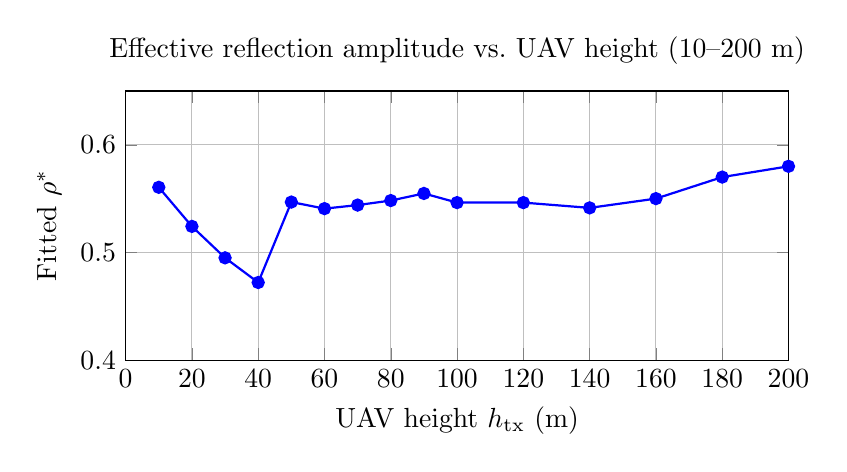
\begin{tikzpicture}
\begin{axis}[
  width=10cm, height=5cm,
  xlabel={UAV height $h_{\mathrm{tx}}$ (m)},
  ylabel={Fitted $\rho^*$},
  xmin=0, xmax=200,
  ymin=0.4, ymax=0.65,
  grid=major,
  title={Effective reflection amplitude vs.\ UAV height (10--200 m)}
]
\addplot[mark=*, thick, blue] coordinates {
  (10,0.5605)(20,0.5242)(30,0.4950)(40,0.4721)
  (50,0.5468)(60,0.5407)(70,0.5440)(80,0.5482)
  (90,0.5548)(100,0.5463)(120,0.5463)(140,0.5414)
  (160,0.55)(180,0.57)(200,0.58)
};
\end{axis}
\end{tikzpicture}
\caption{Effective ground-reflection amplitude $\rho^*$ as a function of UAV
height, fitted independently per 5 m height bin. Values are stable in the
range $0.47$--$0.56$ for 10--130 m, then rise slightly at higher altitudes
where training data is sparser.}
\label{fig:rho_vs_h}
\end{figure}

\begin{figure}[H]
\centering
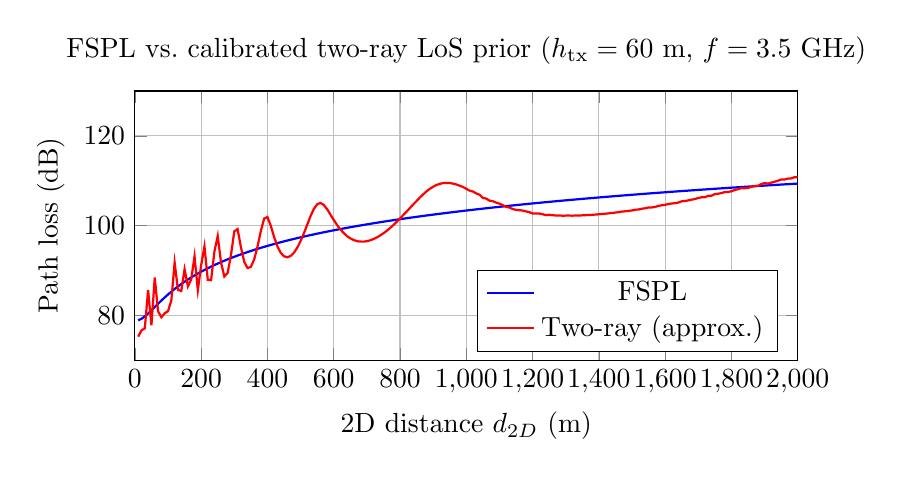
\begin{tikzpicture}
\begin{axis}[
  width=10cm, height=5cm,
  xlabel={2D distance $d_{2D}$ (m)},
  ylabel={Path loss (dB)},
  xmin=0, xmax=2000,
  ymin=70, ymax=130,
  grid=major,
  legend pos=south east,
  title={FSPL vs.\ calibrated two-ray LoS prior ($h_{\mathrm{tx}} = 60$ m, $f = 3.5$ GHz)}
]
\addplot[thick, blue, domain=10:2000, samples=200]
  {32.45 + 20*ln(sqrt(x^2+3481)/1000)/ln(10) + 20*ln(3500)/ln(10)};
\addlegendentry{FSPL}
\addplot[thick, red, domain=10:2000, samples=200]
  {32.45 + 20*ln(sqrt(x^2+3481)/1000)/ln(10) + 20*ln(3500)/ln(10)
   - 20*ln(abs(1 + 0.54 * sqrt(x^2+3481)/sqrt(x^2+3721) *
   cos(deg(2*3.14159*(sqrt(x^2+3721)-sqrt(x^2+3481))*3500e6/3e8))))/ln(10)};
\addlegendentry{Two-ray (approx.)}
\end{axis}
\end{tikzpicture}
\caption{Schematic comparison of FSPL and the coherent two-ray model for a
60 m UAV at 3.5 GHz ($h_{\mathrm{rx}} = 1.5$ m). The two-ray model produces
a characteristic oscillatory pattern around the FSPL baseline, corresponding
to alternating zones of constructive and destructive interference.}
\label{fig:tworay_pl}
\end{figure}

\subsection{NLoS branch}
\label{sec:nlos_branch}

The NLoS path-loss branch used in \texttt{Try 80} is not a pure literature
formula. It is a hybrid engineering model built in four stages.

\subsubsection{Stage 1: raw NLoS propagation prior}

Two coarse physical estimates are combined.

\paragraph{COST-231 term.}
The COST-231 / Hata extension for urban macro cells gives the empirical
large-scale path-loss expression used below \cite{cost231}. It is included
because it is one of the standard references for urban NLoS macrocell loss,
even though the CKM scenario is outside its original frequency and base-station
height range:

\begin{equation}
\begin{aligned}
\mathrm{PL}_{\mathrm{COST231}}(x)
={}&
46.3 + 33.9 \log_{10}(f_{\mathrm{MHz}})
- 13.82 \log_{10}(h_{\mathrm{tx}})
- a(h_{\mathrm{rx}})\\
&+
\left(44.9 - 6.55 \log_{10}(h_{\mathrm{tx}})\right)
\log_{10}(d_{\mathrm{km}})
+ 3
\end{aligned}
\label{eq:cost231}
\end{equation}

where $d_{\mathrm{km}} = d_{2D}(x)/1000$ and the mobile antenna correction
factor for large cities is:

\begin{equation}
a(h_{\mathrm{rx}}) = 3.2(\log_{10}(11.75\,h_{\mathrm{rx}}))^2 - 4.97
\label{eq:cost231_a}
\end{equation}

Equation~\eqref{eq:cost231} should therefore be read as a \emph{shape prior},
not as a trusted absolute predictor. COST-231 contributes the expected
log-distance growth, transmitter-height dependence and receiver-height
correction of an urban empirical model. The subsequent calibration stage is
what adapts that shape to the 7.125 GHz UAV ray-tracing setting used here.

\paragraph{Interpretation of Eq.~\eqref{eq:cost231}.}
\begin{itemize}
\item $46.3 + 33.9\log_{10}(f_{\mathrm{MHz}})$: frequency-dependent offset.
      The exponent $33.9$ (compare to $20$ for FSPL) reflects stronger
      frequency dependence in urban scattering.
\item $-13.82\log_{10}(h_{\mathrm{tx}})$: as the base station / UAV gets
      higher, path loss decreases (better clearance above rooftops). The
      $-13.82$ coefficient is a fitted constant from the Hata empirical
      dataset.
\item $-a(h_{\mathrm{rx}})$: accounts for the receiver height. For typical
      pedestrian heights ($h_{\mathrm{rx}} \approx 1.5$ m), $a \approx
      -0.6$ dB, which is small.
\item $(44.9 - 6.55\log_{10}(h_{\mathrm{tx}}))\log_{10}(d_{\mathrm{km}})$:
      distance-dependent term. The effective path-loss exponent is
      $(44.9 - 6.55\log_{10}(h_{\mathrm{tx}}))/10$, which decreases as the
      UAV climbs (effectively reducing NLoS scattering losses at longer
      distances from higher altitudes).
\item $+3$: the COST-231 metropolitan correction constant (dB), corresponding
      to the dense-urban correction in the original model \cite{cost231}.
\end{itemize}

\paragraph{Elevation-aware UAV envelope.}
The A2G NLoS envelope models the elevation-angle dependence of urban
air-to-ground path loss. The dependence on elevation angle follows the common
UAV channel-model observation that links at larger elevation angles have fewer
obstructions and lower shadowing variance \cite{khawaja_survey,tr38901}.

\begin{equation}
\mathrm{PL}_{\mathrm{A2G,NLoS}}(x)
=
\lambda_0(h_{\mathrm{tx}}, f)
+ \beta_{\mathrm{NLoS}}
+ A_{\mathrm{NLoS}}
\exp\!\left(-\frac{90-\theta^\circ(x)}{\tau_{\mathrm{NLoS}}}\right)
\label{eq:a2g_nlos}
\end{equation}

where:
\begin{align}
\lambda_0(h_{\mathrm{tx}}, f)
&= 20\log_{10}\!\left(\frac{4\pi h_{\mathrm{tx}} f}{c}\right)
\label{eq:lambda0}
\end{align}

The fitted constants are:
$\beta_{\mathrm{NLoS}} = -16.16$ dB,
$A_{\mathrm{NLoS}} = 12.0436$,
$\tau_{\mathrm{NLoS}} = 7.52$ deg.

\paragraph{Interpretation of Eq.~\eqref{eq:a2g_nlos}.}
\begin{itemize}
\item $\lambda_0$: a free-space-like offset that scales with UAV height and
      frequency~\cite{khawaja_survey,wocc2021}. The CKM dataset uses
      $f = 7.125$ GHz (FR2 lower edge per 3GPP NR~\cite{tr38901}); for
      $h_{\mathrm{tx}} = 50$ m at that frequency, $\lambda_0 \approx 103$ dB.
\item $\beta_{\mathrm{NLoS}} = -16.16$ dB: a baseline NLoS attenuation
      offset relative to $\lambda_0$.
\item $A_{\mathrm{NLoS}}\exp(-\ldots)$: an exponential modulation with
      $(90 - \theta^\circ)$. When the elevation angle $\theta^\circ$ is high
      (UAV nearly overhead, $\theta^\circ \to 90^\circ$), the exponent
      vanishes and the term goes to $A_{\mathrm{NLoS}}$. When $\theta^\circ$
      is low (grazing incidence), the exponent is large and the term
      approaches zero. The effect is that NLoS path loss \emph{decreases} as
      the UAV moves overhead, consistent with improved clearance above
      buildings.
\item $\tau_{\mathrm{NLoS}} = 7.52^\circ$: the characteristic angular scale.
      A low value means the transition from grazing to overhead happens
      sharply within a small elevation range.
\end{itemize}

The raw NLoS prior is then the conservative (higher) of the two estimates:

\begin{equation}
\mathrm{PL}_{\mathrm{NLoS,raw}}(x)
=
\max\left(
\mathrm{PL}_{\mathrm{COST231}}(x),
\mathrm{PL}_{\mathrm{A2G,NLoS}}(x)
\right)
\label{eq:nlos_raw}
\end{equation}

The maximum in Eq.~\eqref{eq:nlos_raw} is deliberately pessimistic. If the
empirical COST-231 curve predicts stronger attenuation than the A2G envelope,
the model keeps the urban-macro value; if the elevation-aware envelope predicts
stronger attenuation, the model keeps the A2G value. This prevents the raw
prior from becoming unrealistically optimistic in NLoS streets where neither
source model is fully valid on its own.

The full raw prior blends the LoS and NLoS estimates using the LoS mask
$m_{\mathrm{LoS}}(x) \in [0,1]$:

\begin{equation}
\mathrm{PL}^{(0)}(x)
=
m_{\mathrm{LoS}}(x)\,\mathrm{PL}_{\mathrm{LoS,blend}}(x)
+
\left(1-m_{\mathrm{LoS}}(x)\right)\mathrm{PL}_{\mathrm{NLoS,raw}}(x)
\label{eq:pl0}
\end{equation}

with a soft blend for the LoS branch:

\begin{equation}
\mathrm{PL}_{\mathrm{LoS,blend}}(x)
=
0.7\,\mathrm{PL}_{\mathrm{LoS,path}}(x)
+0.3\min\left(\mathrm{PL}_{\mathrm{LoS,path}}(x), \mathrm{PL}_{\mathrm{A2G,LoS}}(x)\right)
\label{eq:los_blend}
\end{equation}

The $0.7/0.3$ blend in Eq.~\eqref{eq:los_blend} gives 70\% weight to the
two-ray LoS model and 30\% weight to the minimum of the two-ray model and an
A2G LoS envelope. This prevents the prediction from exceeding a physically
motivated upper bound in the LoS case.

\subsubsection{Stage 2: map-derived morphology features}

From $\mathrm{PL}^{(0)}(x)$ and the map topology, a 15-element feature
vector is computed:

\begin{equation}
\textbf{x}_{78}(x)
=
\begin{bmatrix}
\mathrm{PL}^{(0)}(x)^2 \\
\mathrm{PL}^{(0)}(x) \\
\log(1+d_{2D}(x)) \\
\rho_{15}(x) \\
\rho_{41}(x) \\
h_{15}(x) \\
h_{41}(x) \\
\rho_{41}(x)\log(1+d_{2D}(x)) \\
n_{15}(x) \\
n_{41}(x) \\
n_{41}(x)\log(1+d_{2D}(x)) \\
\sigma_{\mathrm{shadow}}(x) \\
\theta_{\mathrm{norm}}(x) \\
n_{41}(x)\theta_{\mathrm{norm}}(x) \\
1
\end{bmatrix}
\label{eq:x78}
\end{equation}

The lowercase bold notation is intentional: \(\textbf{x}_{78}(x)\) is a
per-pixel feature vector. When vectors from many pixels in one regime are
stacked for calibration, they form the uppercase design matrix
\(\textbf{X}_r\). Table~\ref{tab:x78_term_inventory} gives the role of each
entry before the detailed definitions below.

\begin{table}[H]
\centering
\small
\begin{tabularx}{\textwidth}{p{3.1cm} X X}
\toprule
\textbf{Term} & \textbf{Mathematical role} & \textbf{Physical interpretation} \\
\midrule
\(\mathrm{PL}^{(0)}(x)^2\) & Quadratic basis term. & Lets the linear calibration bend the raw path-loss curve when the raw model is systematically curved. \\
\(\mathrm{PL}^{(0)}(x)\) & Linear raw-prior term. & Keeps the calibrated model anchored to the physical prior instead of relearning path loss from scratch. \\
\(\log(1+d_{2D}(x))\) & Smooth distance basis. & Mirrors log-distance propagation laws used in classical models \cite{rappaport,cost231}. \\
\(\rho_{15}(x),\rho_{41}(x)\) & Local building-density averages. & Count how much nearby urban structure can block, reflect or diffract the signal. \\
\(h_{15}(x),h_{41}(x)\) & Density-weighted local height averages. & Distinguish low dense blocks from taller blocks with stronger obstruction. \\
\(\rho_{41}(x)\log(1+d_{2D}(x))\) & Density-distance interaction. & Allows distance slope to increase in dense areas. \\
\(n_{15}(x),n_{41}(x)\) & Local NLoS-support fractions. & Measure how much nearby ground is geometrically shielded from the UAV. \\
\(n_{41}(x)\log(1+d_{2D}(x))\) & NLoS-distance interaction. & Allows blocked streets to accumulate loss differently with range. \\
\(\sigma_{\mathrm{shadow}}(x)\) & Elevation-dependent shadowing proxy. & Encodes the stronger low-elevation variability reported in A2G channel models \cite{khawaja_survey,tr38901}. \\
\(\theta_{\mathrm{norm}}(x)\) & Normalized elevation angle. & Separates grazing links from near-overhead links. \\
\(n_{41}(x)\theta_{\mathrm{norm}}(x)\) & NLoS-elevation interaction. & Allows the NLoS correction to depend on whether shielding occurs at low or high elevation. \\
\(1\) & Bias term. & Lets each regime learn a constant offset after all physical terms are included. \\
\bottomrule
\end{tabularx}
\caption{Term-by-term inventory of the \texttt{Try 78} calibration vector.}
\label{tab:x78_term_inventory}
\end{table}

Each term is now described in detail.

\paragraph{Base masks.}
The ground mask is:

\begin{equation}
g(x)=
\begin{cases}
1, & \text{if } \mathrm{topology}(x)=0 \\
0, & \text{otherwise}
\end{cases}
\label{eq:ground_mask_v2}
\end{equation}

The building mask is $b(x)=1-g(x)$.
The ground-NLoS support mask is:

\begin{equation}
n_{\mathrm{raw}}(x)=
\mathbb{1}\!\left[m_{\mathrm{LoS}}(x)\le 0.5\right]\cdot g(x)
\label{eq:nlos_mask_v2}
\end{equation}

This selects ground pixels that are predominantly in NLoS, i.e., pixels that
are at street level and are shielded from the UAV.

\paragraph{Quadratic raw-prior feature.}
The pair $(\mathrm{PL}^{(0)}(x)^2, \mathrm{PL}^{(0)}(x))$ allows the linear
model to fit a \emph{quadratic} relationship in the raw prior. Including both
$P^2$ and $P$ as features lets the calibration curve be:
$\hat P = \beta_1 P^2 + \beta_2 P + \cdots$, which can correct for
systematic curvature in the raw prior.

\paragraph{Distance term.}
$\log(1+d_{2D}(x))$: the logarithm of one plus the horizontal distance,
providing a distance-dependent offset. The $+1$ prevents a singularity at
$d_{2D}=0$.
The logarithm is consistent with the log-distance structure of empirical
path-loss laws: a multiplicative increase in distance produces an additive
increase in predicted dB loss \cite{rappaport,cost231}.

\paragraph{Per-pixel box-mean operator.}
\label{par:boxmean}

All multiscale features use the same 2D box-mean operator
$\mathrm{BoxMean}_k$. For a map $f : \mathbb{Z}^2 \to \mathbb{R}$ and a
window half-width $p = \lfloor k/2 \rfloor$, the value at pixel
$x = (i, j)$ is:

\begin{equation}
\mathrm{BoxMean}_k(f)(i,j)
=
\frac{1}{k^2}
\sum_{i'=i-p}^{i+p}\,\sum_{j'=j-p}^{j+p}
f_{\mathrm{padded}}(i',j')
\label{eq:boxmean}
\end{equation}

where $f_{\mathrm{padded}}$ is $f$ extended outside the map boundary by
\emph{reflect} (mirror) padding: $f_{\mathrm{padded}}(-r, j) =
f_{\mathrm{padded}}(r, j)$ and similarly at all four edges. This ensures
border pixels receive a full $k^2$-pixel average, with the map reflected back
inward rather than zero-padded.

Equation~\eqref{eq:boxmean} is evaluated efficiently using a
\emph{2D summed-area table} (integral image). Let $I(i,j)=\sum_{i'\le
i, j'\le j} f_{\mathrm{padded}}(i',j')$ be the prefix-sum array. Then:

\begin{equation}
\sum_{i'=i-p}^{i+p}\sum_{j'=j-p}^{j+p} f_{\mathrm{padded}}(i',j')
=
I(i+p,\,j+p)
-I(i-p-1,\,j+p)
-I(i+p,\,j-p-1)
+I(i-p-1,\,j-p-1)
\label{eq:sat}
\end{equation}

This reduces each per-pixel evaluation to four table lookups, making the
full-map computation $O(HW)$ regardless of $k$. In the implementation,
$k \in \{15, 41\}$ pixels, corresponding to $\sim$15 m and $\sim$41 m
neighborhoods (1 m/pixel resolution).

\paragraph{Multiscale building density.}

\begin{equation}
\rho_k(x)=\mathrm{BoxMean}_k\!\left(b(\cdot)\right)(x)
=
\frac{1}{k^2}\sum_{x' \in W_k(x)} b(x')
\label{eq:rho_k}
\end{equation}

where $W_k(x)$ is the $k\times k$ window centered at $x$.
Since $b(x') \in \{0,1\}$, $\rho_k(x)$ is the \emph{fraction of pixels
that are buildings} in the window. It is zero at a ground pixel
surrounded only by other ground pixels, and one at a pixel deep inside a
solid building block. $\rho_{15}$ captures fine-scale building density within
a $\sim$15 m neighborhood; $\rho_{41}$ captures a coarser $\sim$41 m
neighborhood.

\paragraph{Multiscale building height.}

\begin{equation}
h_k(x)=
\frac{\mathrm{BoxMean}_k\!\left(\mathrm{topology}(\cdot)\,b(\cdot)\right)(x)}
{H_{\mathrm{norm}}},
\quad H_{\mathrm{norm}} = 90 \;\mathrm{m}
\label{eq:h_k}
\end{equation}

This is the box mean of $\mathrm{topology}(x')\cdot b(x')$:
building pixels contribute their height in metres; ground pixels contribute
0. Dividing by $k^2$ (inside $\mathrm{BoxMean}_k$) gives:

\begin{equation}
h_k(x)=
\frac{1}{H_{\mathrm{norm}}\,k^2}
\sum_{x'\in W_k(x)}
\mathrm{topology}(x')\cdot b(x')
=
\frac{\rho_k(x)}{H_{\mathrm{norm}}}\;\overline{h}_{\mathrm{bldg},k}(x)
\label{eq:h_k_interp}
\end{equation}

where $\overline{h}_{\mathrm{bldg},k}(x)$ is the \emph{mean height of
building pixels only} within the window:

\begin{equation}
\overline{h}_{\mathrm{bldg},k}(x)
=
\frac{\displaystyle\sum_{x'\in W_k(x)} \mathrm{topology}(x')\,b(x')}
     {\displaystyle\sum_{x'\in W_k(x)} b(x')}
\quad\text{(undefined if }\rho_k(x)=0\text{)}
\label{eq:mean_bldg_height}
\end{equation}

Critically, $h_k(x) = \rho_k(x)\cdot\overline{h}_{\mathrm{bldg},k}(x)/H_{\mathrm{norm}}$,
so $h_k$ combines \emph{both} how many buildings are present and how tall they
are. A window with 50\% building coverage and mean height 20 m gives the same
$h_k$ as a window with 100\% coverage at mean height 10 m. The $H_{\mathrm{norm}}
= 90$ m normalizer maps the joint range to approximately $[0, 1]$.

\paragraph{Multiscale NLoS-support.}

\begin{equation}
n_k(x)=\mathrm{BoxMean}_k\!\left(n_{\mathrm{raw}}(\cdot)\right)(x)
\label{eq:n_k}
\end{equation}

Since $n_{\mathrm{raw}}(x') \in \{0,1\}$ (Eq.~\ref{eq:nlos_mask_v2}),
$n_k(x)$ is the \emph{absolute fraction of the window area} that consists of
ground pixels in NLoS. Just as $h_k(x)$ conflates building coverage and building
height, $n_k(x)$ conflates ground coverage and NLoS probability. We can write:

\begin{equation}
n_k(x)
=
\left(1 - \rho_k(x)\right)
\overline{n}_{\mathrm{ground}, k}(x)
\label{eq:n_k_interp}
\end{equation}

where $\overline{n}_{\mathrm{ground}, k}(x)$ is the relative fraction of
\emph{available ground pixels} that are shielded:

\begin{equation}
\overline{n}_{\mathrm{ground}, k}(x)
=
\frac{\displaystyle\sum_{x'\in W_k(x)} n_{\mathrm{raw}}(x')}
     {\displaystyle\sum_{x'\in W_k(x)} g(x')}
\quad\text{(undefined if }\rho_k(x)=1\text{)}
\end{equation}

Because building pixels never contribute to $n_k$, this feature is zero in
completely open LoS areas (where $\overline{n}_{\mathrm{ground}, k} = 0$)
\emph{and} deep inside solid building blocks (where $1 - \rho_k = 0$). It
reaches its maximum in narrow urban street canyons, where ground coverage is
still significant but entirely shielded from the UAV.

\paragraph{Elevation angle.}

\begin{equation}
\theta(x)=\arctan\left(\frac{h_{\mathrm{tx}}-h_{\mathrm{rx}}}{\max(d_{2D}(x),1)}\right)
\label{eq:theta_v2}
\end{equation}

The $\max(\cdot, 1)$ prevents division by zero directly below the UAV.
Then:

\begin{equation}
\theta_{\mathrm{norm}}(x)=
\mathrm{clip}\left(\frac{\theta^\circ(x)}{90},\,0,\,1\right)
\label{eq:theta_norm_v2}
\end{equation}

where $\theta^\circ = \theta \cdot 180/\pi$ is in degrees. $\theta_{\mathrm{norm}}
= 0$ at grazing incidence, $= 1$ directly overhead.

\paragraph{Shadowing proxy.}

\begin{align}
\sigma_{\mathrm{LoS}}(x) &= \alpha_{\mathrm{LoS}}\,(90-\theta^\circ(x))^{\mu_{\mathrm{LoS}}}
\label{eq:sigma_los_v2}\\
\sigma_{\mathrm{NLoS}}(x) &= \alpha_{\mathrm{NLoS}}\,(90-\theta^\circ(x))^{\mu_{\mathrm{NLoS}}}
\label{eq:sigma_nlos_v2}
\end{align}

with fitted values $\alpha_{\mathrm{NLoS}} = 2.3197$, $\mu_{\mathrm{NLoS}}
= 0.2361$. The blended proxy is:

\begin{equation}
\sigma_{\mathrm{shadow}}(x)=
m_{\mathrm{LoS}}(x)\,\sigma_{\mathrm{LoS}}(x)
+\left(1-m_{\mathrm{LoS}}(x)\right)\sigma_{\mathrm{NLoS}}(x)
\label{eq:sigma_blend}
\end{equation}

This acts as a spatially varying uncertainty proxy: higher values at low
elevation angles, where propagation conditions are more difficult.

\paragraph{Interaction terms.}
The three pairwise products
$\rho_{41}(x)\log(1+d_{2D}(x))$,
$n_{41}(x)\log(1+d_{2D}(x))$, and
$n_{41}(x)\theta_{\mathrm{norm}}(x)$
allow the linear model to capture effects where building density or NLoS
support \emph{modifies} the slope of path loss with distance or elevation
angle, rather than just shifting it.

\subsubsection{Stage 3: regime-wise linear calibration}

The regime $r$ is identified by three keys:
\begin{itemize}
\item \emph{Coarse topology:} one of \texttt{open\_lowrise},
      \texttt{mixed\_midrise}, or \texttt{dense\_highrise},
\item \emph{Propagation state:} \texttt{LoS} or \texttt{NLoS},
\item \emph{Antenna height bin:} \texttt{low\_ant}, \texttt{mid\_ant}, or
      \texttt{high\_ant}.
\end{itemize}
This gives up to $3 \times 2 \times 3 = 18$ regimes.

\paragraph{How topology class and antenna bin are computed.}
These are \emph{per-map} scalar labels, not per-pixel quantities.
They are derived once from the full topology tensor and UAV height.

The \emph{map-level} building density and mean building height are:

\begin{align}
\bar\rho_{\mathrm{map}}
&= \frac{1}{HW}\sum_{x} b(x)
\label{eq:global_density}\\[4pt]
\bar h_{\mathrm{map}}
&= \frac{\displaystyle\sum_{x} \mathrm{topology}(x)\,b(x)}
        {\displaystyle\sum_{x} b(x)}
\label{eq:global_mean_bldg_height}
\end{align}

$\bar\rho_{\mathrm{map}}$ is simply the fraction of map pixels that are
buildings. $\bar h_{\mathrm{map}}$ is the mean building height
\emph{over building pixels only} (the denominator excludes ground pixels).
This is different from the per-pixel feature $h_k(x)$ in
Eq.~\eqref{eq:h_k_interp}, which divides the same numerator by the full
window area $k^2$ instead of by the number of building pixels.

The six topology classes are assigned by thresholding both quantities:

\begin{equation}
\mathrm{class}_6 =
\begin{cases}
\texttt{open\_sparse\_lowrise}   & \bar\rho \le d_1,\; \bar h \le h_1 \\
\texttt{open\_sparse\_vertical}  & \bar\rho \le d_1,\; \bar h > h_1 \\
\texttt{dense\_block\_midrise}   & \bar\rho \ge d_2,\; \bar h \le h_2 \\
\texttt{dense\_block\_highrise}  & \bar\rho \ge d_2,\; \bar h > h_2 \\
\texttt{mixed\_compact\_lowrise} & d_1 < \bar\rho < d_2,\; \bar h \le h_1 \\
\texttt{mixed\_compact\_midrise} & d_1 < \bar\rho < d_2,\; \bar h > h_1
\end{cases}
\label{eq:topo6}
\end{equation}

with thresholds $d_1 = 0.12$, $d_2 = 0.28$ (density fractions),
$h_1 = 12$ m, $h_2 = 28$ m. The three-class label
(\texttt{open}/\texttt{mixed}/\texttt{dense}) is the prefix of
$\mathrm{class}_6$ and is used in \texttt{Try 80} reporting.

The antenna-height bin is assigned by UAV height tertiles:

\begin{equation}
\mathrm{ant\_bin} =
\begin{cases}
\texttt{low\_ant}  & h_{\mathrm{tx}} \le 58.12\;\mathrm{m} \\
\texttt{mid\_ant}  & 58.12 < h_{\mathrm{tx}} \le 103.85\;\mathrm{m} \\
\texttt{high\_ant} & h_{\mathrm{tx}} > 103.85\;\mathrm{m}
\end{cases}
\label{eq:ant_bin_v2}
\end{equation}

The calibrated prediction for regime $r$ is:
\begin{equation}
\widehat{\mathrm{PL}}_{r}(x)
=
\textbf{x}_{78}(x)^\top \textbf{w}^{78}_{r}
=
\sum_{j=1}^{15} x_j(x)\,w^{78}_{r,j}
\label{eq:pl_cal}
\end{equation}

\paragraph{How $\textbf{w}^{78}_{r}$ is fitted.}
Across all training samples whose regime label equals $r$, a linear
regression is run:

\begin{equation}
\hat{\textbf{w}}^{78}_{r}
=
\arg\min_{\textbf{w}\in\mathbb{R}^{15}} \sum_{x \in \mathcal{S}_r} \left(y(x) - \textbf{x}_{78}(x)^\top \textbf{w}\right)^2
\label{eq:ols}
\end{equation}

where $\mathcal{S}_r$ is the set of all valid pixels in training samples
belonging to regime $r$. This ordinary least squares problem has the closed
form solution:

\begin{equation}
\hat{\textbf{w}}^{78}_{r}
=
\left(\textbf{X}_r^\top \textbf{X}_r\right)^{-1}
\textbf{X}_r^\top \textbf{y}_r
\label{eq:ols_closed}
\end{equation}

where $\textbf{X}_r$ stacks the feature vectors and $\textbf{y}_r$ stacks
the measured path-loss values. In practice, if the matrix is near-singular
(sparse regime), a fallback to a less specific regime key is used (see
the fallback chain in the Try 79 section, which uses the same strategy).

The terms in Eq.~\eqref{eq:ols_closed} are standard linear least-squares
quantities. The matrix \(\textbf{X}_r^\top\textbf{X}_r\) is the
\emph{Gram matrix}; its diagonal entries measure the energy of each feature
inside regime \(r\), and its off-diagonal entries measure correlations between
features. The vector \(\textbf{X}_r^\top\textbf{y}_r\) measures how strongly
each feature correlates with measured path loss. The inverse maps those
feature-target correlations into the fitted coefficient vector
\(\hat{\textbf{w}}^{78}_{r}\). This is the classical ordinary least-squares
solution, but applied separately per propagation regime rather than globally.

An example fitted coefficient vector for the \texttt{mixed\_midrise|LoS|high\_ant}
regime is:
\[
\textbf{w}^{78}_{\texttt{mixed|LoS|high}}
=
\begin{bmatrix}
-0.000554,\ 0.761,\ 3.061,\ 0.127,\ 0.793,\ -2.318,\ -0.481,\ -0.157 \\[4pt]
0.155,\ -0.218,\ 0.060,\ -47.15,\ -28.08,\ -0.508,\ 48.83
\end{bmatrix}^\top
\]
The large bias weight ($w_{15} = 48.83$) and the large negative
shadowing-proxy weight ($w_{12} = -47.15$) partially cancel, together
acting as a calibrated effective offset for this regime.

\subsubsection{Stage 4: region replacement and clipping}

\begin{equation}
\mathrm{PL}_{\mathrm{NLoS}}(x)
=
\mathrm{clip}\!\left(
\textbf{x}_{78}(x)^\top \textbf{w}^{78}_{r},
20,
180
\right)
\label{eq:pl_nlos_final}
\end{equation}

Hard clipping to $[20, 180]$ dB prevents the linear model from producing
physically unreasonable values. The final hybrid path-loss prior is:

\begin{equation}
\mathrm{PL}_{\mathrm{prior}}(x)
=
\begin{cases}
\mathrm{PL}_{\mathrm{LoS}}(x), & m_{\mathrm{LoS}}(x) > 0.5 \\
\mathrm{PL}_{\mathrm{NLoS}}(x), & \text{otherwise}
\end{cases}
\label{eq:pl_hybrid}
\end{equation}

\subsection{Evaluation metric: pixel-weighted RMSE}

\label{sec:pw_metric}

All numerical results are reported as \emph{pixel-weighted} (pw) RMSE or MAE.
Building pixels ($\mathrm{topology}(x) > 0$) are always excluded; only valid
ground pixels with a finite, physically plausible target value contribute.
Let $\mathcal{V}_k$ be the set of all such valid $(s, x)$ pairs across all
evaluation samples for task $k$. Then:

\begin{equation}
\mathrm{RMSE}^{\mathrm{pw}}_k
=
\sqrt{
  \frac{\displaystyle\sum_{(s,x)\in\mathcal{V}_k}
  \left(\hat{y}_k^{(s)}(x) - y_k^{(s)}(x)\right)^2}
  {\displaystyle|\mathcal{V}_k|}
}
\label{eq:rmse_pw_v2}
\end{equation}

This is a single square root over all pooled valid pixels, not an average of
per-sample RMSEs. Units are dB (path loss), ns (delay spread), and
degrees (angular spread), all in the native non-transformed domain.

\subsection{Observed Try 78 results}

Table~\ref{tab:try78_rmse} summarizes the path-loss RMSE values obtained from
the final hybrid evaluation.

\begin{table}[H]
\centering
\caption{Try 78 pixel-weighted RMSE (dB) on the evaluation split. The
``Role'' column indicates whether the model is used as a frozen prior in
\texttt{Try 80}, serves only as an ablation baseline, or is an intermediate
construction step.}
\label{tab:try78_rmse}
\begin{tabular}{lcc}
\toprule
Model & RMSE (dB) & Role in Try 80\\
\midrule
FSPL (LoS only)            & 3.9540 & ablation baseline (not used)\\
FSPL + radial residual     & 3.7086 & ablation baseline (not used)\\
Coherent two-ray (LoS)     & 1.7516 & building block $\to$ folded into Hybrid LoS\\
Hybrid LoS                 & 1.7516 & \textbf{frozen LoS prior} (used in Try 80)\\
Hybrid NLoS                & 3.3967 & \textbf{frozen NLoS prior} (used in Try 80)\\
\midrule
\textbf{Hybrid overall}    & \textbf{1.9246} & combined frozen prior (Try 80 input)\\
\bottomrule
\end{tabular}
\end{table}

\paragraph{Why do Coherent two-ray (LoS) and Hybrid LoS show the same RMSE?}
The two rows report the same value (1.7516 dB) on the \emph{evaluation split},
but they are not identical models.

\begin{itemize}
\item \textbf{Coherent two-ray (LoS)} is the standalone two-ray model
      (Eq.~\ref{eq:pl_los}) applied only to LoS pixels, with no soft clipping
      from an A2G envelope.
\item \textbf{Hybrid LoS} applies the blend of Eq.~\ref{eq:los_blend}:
      $0.7\,\mathrm{PL}_{\mathrm{LoS,path}} + 0.3\min(\mathrm{PL}_{\mathrm{LoS,path}},
      \mathrm{PL}_{\mathrm{A2G,LoS}})$.
      For the vast majority of pixels the two-ray prediction is already below
      the A2G LoS envelope, so the $\min$ resolves to the two-ray value and
      the blend collapses to $0.7P + 0.3P = P$. The two formulas therefore
      coincide on almost all evaluation pixels, producing the same aggregate RMSE.
\end{itemize}

The practical difference only surfaces on pixels where the two-ray model
predicts \emph{unrealistically low} path loss (constructive-interference peaks
that overshoot the measurement). On those pixels the A2G envelope acts as a
physical upper-bound cap, slightly raising the prediction and preventing it
from being overly optimistic. On the training set, where such edge cases
appear more frequently, Hybrid LoS was marginally better than the standalone
two-ray; the improvement rounds away at the reported precision for the
evaluation split. The hybrid formulation was therefore kept as the frozen LoS
prior in \texttt{Try 80} because it is more conservative and physically
bounded, even though the difference is not visible at this precision.

\begin{figure}[H]
\centering
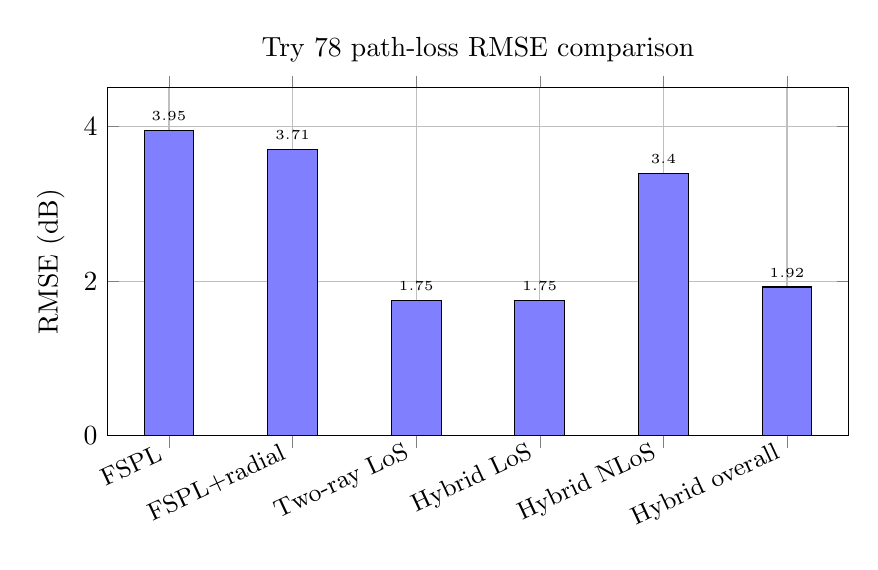
\begin{tikzpicture}
\begin{axis}[
  ybar,
  width=11cm, height=6cm,
  bar width=18pt,
  ylabel={RMSE (dB)},
  symbolic x coords={FSPL,FSPL+radial,Two-ray LoS,Hybrid LoS,Hybrid NLoS,Hybrid overall},
  xtick=data,
  x tick label style={rotate=25, anchor=east, font=\small},
  ymin=0, ymax=4.5,
  nodes near coords,
  nodes near coords align={vertical},
  every node near coord/.append style={font=\tiny},
  grid=major,
  title={Try 78 path-loss RMSE comparison}
]
\addplot[fill=blue!50] coordinates {
  (FSPL,3.9540)
  (FSPL+radial,3.7086)
  (Two-ray LoS,1.7516)
  (Hybrid LoS,1.7516)
  (Hybrid NLoS,3.3967)
  (Hybrid overall,1.9246)
};
\end{axis}
\end{tikzpicture}
\caption{Try 78 pixel-weighted RMSE values. The coherent two-ray model
reduces LoS RMSE from 3.95 dB (FSPL) to 1.75 dB, a gain of 2.2 dB.}
\label{fig:try78_rmse}
\end{figure}

\begin{figure}[H]
\centering
\begin{tikzpicture}[
    >=stealth,
    node distance=1cm and 2cm,
    block/.style={draw, thick, fill=blue!10, rectangle, rounded corners, minimum width=3.5cm, minimum height=1cm, align=center},
    input/.style={draw, thick, fill=gray!20, rectangle, minimum width=2.5cm, minimum height=0.8cm, align=center},
    sum/.style={draw, thick, fill=green!10, rectangle, rounded corners, minimum width=3.5cm, minimum height=1cm, align=center},
    branch/.style={draw, thick, fill=orange!10, rectangle, rounded corners, minimum width=3.5cm, minimum height=1cm, align=center}
]

% Inputs
\node[input] (geom) {Geometry \\ $d_{2D}, \theta, h_{\mathrm{tx}}, h_{\mathrm{rx}}$};
\node[input, right=4cm of geom] (map) {CKM Map \\ $b(x), g(x), m_{\mathrm{LoS}}(x)$};

% LoS Branch
\node[block, below left=1.5cm and 0.5cm of geom] (fspl) {FSPL \\ (Eq.~\ref{eq:fspl})};
\node[block, below=1.5cm of fspl] (tworay) {Coherent Two-Ray \\ $C_{\mathrm{2ray}}(x)$};
\node[block, below=1.5cm of tworay] (bias_rad) {Bias + Radial Residual \\ $b + r(d_{2D})$};
\node[branch, below=1.5cm of bias_rad] (pl_los) {Calibrated LoS \\ $\mathrm{PL}_{\mathrm{LoS}}(x)$};

\draw[->, thick] (geom.south) ++(-1,0) |- node[pos=0.75, above, font=\scriptsize] {$\mathbb{R}^{H \times W}$} (fspl.east);
\draw[->, thick] (fspl) -- node[right, font=\scriptsize] {$\mathbb{R}^{H \times W}$} (tworay);
\draw[->, thick] (tworay) -- node[right, font=\scriptsize] {$\mathbb{R}^{H \times W}$} (bias_rad);
\draw[->, thick] (bias_rad) -- node[right, font=\scriptsize] {$\mathbb{R}^{H \times W}$} (pl_los);

% NLoS Branch
\node[block, below right=1.5cm and 0.5cm of geom] (raw_nlos) {Raw NLoS Prior \\ $\max(\text{COST231}, \text{A2G})$};
\node[block, below=1.5cm of raw_nlos] (feat78) {Morphology Features \\ $\textbf{x}_{78}(x) \in \mathbb{R}^{15}$};
\node[block, below=1.5cm of feat78] (ols) {Regime-wise OLS \\ $\textbf{x}_{78}(x)^\top \hat{\textbf{w}}^{78}_{r}$};
\node[branch, below=1.5cm of ols] (pl_nlos) {Calibrated NLoS \\ $\mathrm{PL}_{\mathrm{NLoS}}(x)$};

\draw[->, thick] (geom.south) ++(1,0) |- node[pos=0.75, above, font=\scriptsize] {$\mathbb{R}^{H \times W}$} (raw_nlos.west);
\draw[->, thick] (map.south) |- node[pos=0.75, above, font=\scriptsize] {$\mathbb{R}^{3 \times H \times W}$} (feat78.east);
\draw[->, thick] (raw_nlos) -- node[right, font=\scriptsize] {$\mathbb{R}^{H \times W}$} (feat78);
\draw[->, thick] (feat78) -- node[right, font=\scriptsize] {$\mathbb{R}^{15 \times H \times W}$} (ols);
\draw[->, thick] (ols) -- node[right, font=\scriptsize] {$\mathbb{R}^{H \times W}$} (pl_nlos);

% Blend
\node[sum, below right=1cm and 0.5cm of pl_los] (blend) {Switch on \\ $m_{\mathrm{LoS}}(x)$};
\node[input, below=1cm of blend] (final) {Hybrid Path Loss Prior \\ $\mathrm{PL}_{\mathrm{prior}}(x)$};

\draw[->, thick] (pl_los.south) |- node[pos=0.75, above, font=\scriptsize] {$\mathbb{R}^{H \times W}$} (blend.west);
\draw[->, thick] (pl_nlos.south) |- node[pos=0.75, above, font=\scriptsize] {$\mathbb{R}^{H \times W}$} (blend.east);
\draw[->, thick] (blend) -- node[right, font=\scriptsize] {$\mathbb{R}^{H \times W}$} (final);

\end{tikzpicture}
\caption{Pipeline for the \texttt{Try 78} hybrid path loss prior. The LoS branch relies on an explicit two-ray interference model, while the NLoS branch calibrates a raw prior against map-derived morphology features using regime-wise OLS. The two branches are hard-switched based on the LoS mask to produce the final frozen prior.}
\label{fig:try78_pipeline}
\end{figure}
